%%%%%%%%%%%%%%%%%%%%%%%%%%%%%%%%%%%%
% This is the template for submission to ISCA 2019
% The cls file is a modified from  'sig-alternate.cls'
%%%%%%%%%%%%%%%%%%%%%%%%%%%%%%%%%%%%

\documentclass{sig-alternate} 
\usepackage{mathptmx} % This is Times font

\newcommand{\ignore}[1]{}
\usepackage{fancyhdr}
\usepackage[normalem]{ulem}
\usepackage[hyphens]{url}
\usepackage{microtype}

% addtional packages
\usepackage{todonotes}

% Always include hyperref last
\usepackage[bookmarks=true,breaklinks=true,letterpaper=true,colorlinks,linkcolor=black,citecolor=blue,urlcolor=black]{hyperref}

% Ensure letter paper
\pdfpagewidth=8.5in
\pdfpageheight=11in


%%%%%%%%%%%---SETME-----%%%%%%%%%%%%%
\newcommand{\iscasubmissionnumber}{NaN}
%%%%%%%%%%%%%%%%%%%%%%%%%%%%%%%%%%%%

\fancypagestyle{firstpage}{
  \fancyhf{}
\renewcommand{\headrulewidth}{0pt}
  \fancyhead[C]{\normalsize{ISCA 2020 Submission
      \textbf{\#\iscasubmissionnumber} \\ Confidential Draft: DO NOT DISTRIBUTE}} 
  \fancyfoot[C]{\thepage}
}  

\pagenumbering{arabic}

%%%%%%%%%%%---SETME-----%%%%%%%%%%%%%
\title{Processing-in-Memory for Genome Analysis: A Heterogeneous Approach} 
\author{}
%%%%%%%%%%%%%%%%%%%%%%%%%%%%%%%%%%%%

\begin{document}
\maketitle
\thispagestyle{firstpage}
\pagestyle{plain}

\begin{abstract}

This document is intended to serve as a sample for submissions to ISCA 2019. We provide some guidelines that authors should follow when submitting papers to the conference. In an effort to respect the efforts of reviewers and in the interest of fairness to all prospective authors, we request that all submissions follow the formatting and submission rules detailed below. 

\end{abstract}

\section{Introduction}
\todo[inline, color=red!40]{xxxxxxx}


Precision medicine has becoming a promising and efficient approach to clinical diagnoses, allowing patients to be treated with personalized medicine based on a genetic understanding of their disease. For instance, those with leukemia, breast, lung, colon, and rectal cancers are usually tested for certain genetic changes if they develop melanoma..~\cite{shendure2008next,chang2016smem,cong2017aim}. It is predicted that by 2025, 1 billion people will have their own genomes, generating up to 40 exabytes a year of genomic data. This data in turn has led to a plethora of genetic analysis tools~\cite{li2013aligning,li2009sequence,McKenna01092010,picard,SMALT}. Table I depicts three typical genomic analysis flows~\cite{hiseq}. Whole-Genome Sequencing (WGS) provides a base-by-base view of the mutations while Whole-Exome Sequencing (WES) only identifies the coding mutations in cancer, which are less than 2\% of the genome and most likely to contain mutations. Panel targeted special mutations in a given sample.

To keep up with this data deluge, previous studies have focused on providing large-scale or in-memory software framework~\cite{HugeSeq,Massie:EECS-2013-207}. However, using traditional large-scale computing systems will lead to an unaffordable cost of personalized medicine which is advocated to benefit the mass. Furthermore, traditional computer architecture composes of heavy-weight cores and large on-chip caches, which needs to move the massive amount of genomic data from memory to CPU. Another approach is using specialized on-chip accelerators for a particular algorithm or operations case-by-case~\cite{ahmed2015heterogeneous, houtgast2016gpu, liu2012evaluation,chang2016smem, fernandez2011string}. However, these approaches face two challenges. The first challenge is \textit{how to find the next acceleration targets?} As shown in Table I, different scenarios and use cases often necessitate different application combinations. There is a surprising lack of research on the interactions of comprehensive genomic applications with the underlying microarchitecutre. The second challenge is that \textit{system performance is limited by the main memory capacity and bandwidth per server.} Due to the pin count limitation per chip, For instance, Kocberber et al.~\cite{Kocberber:2013bb} observed that using more than four index traversal units. Wang et al.~\cite{yuanrong} observed that using more than 48 PEs do not provide additional speedup due to off-chip bandwidth limitations. Genomic workloads are known to put more pressure on memory bandwidth due to 1) large amounts of random memory access across large input data, which reduces the efficiency of cache system; 2) small computations per loci. These two reasons make it difficult to dig the inherent parallelism of genomic applications with memory hierarchy on conventional architecture.

To provide a higher effective memory bandwidth, processing-in-memory (PIM) and near data processing (NDP) architectures presents new opportunities by integrating compute-logic near memory. 
The recent advancement in integrated circuit (IC) process technology makes these architectures feasible, specifically that of 3D stacking process technology~\cite{zhu2013accelerating,Neurocube,GraphPIM,3Dstacking}.
Hybrid memory cube (HMC)~\cite{HMCSpec}, high bandwidth memory (HBM)~\cite{HBMSpec} are promising memory designs that leverage the benefits of 3D stacking. Such stacked present a viable alternative for addressing this bottleneck leveraging on many processing cores embedded into DRAM. The key objective of adopting PIM is not solely to provide high memory bandwidth, but also to increase scalability for well designed parallel algorithms. In comparison with the integration of compute-logic on the base die, PIM allows the CPU to dispatch parts of the application for execution on compute units that are close to DRAM. Offloading computation using PIM has two major benefits. First, it eliminates a significant portion of the data movement between main memory and conventional processors. Second, it can take advantage of the high-bandwidth and low-latency access to the data inside 3D-stacked DRAM.

The goal of this paper is understanding and mitigating data movement bottlenecks for genomic workloads. We show that the processing-in-memory (PIM) can be a key enabler to realize memory-capacity-proportional performance in large-scale genomic processing under the current pin count limitation. By putting computation logic units on the logic die of 3D-stacked memory, latency and energy overheads of moving data between computation units and main memory can be reduced as well. To investigate the potential benefits of PIM, we first extract commonly used kernels from different genome analysis pipelines, as they account for a significant of the flow execution time. An entire genomic analysis flow can be expressed in a combination of several kernels. Using kernels to express applications is highly intuitive, allowing architecture designers to focus on the behaviors of kernels. We extracted commonly used kernels such as hash-based, fm-index, graph traversal, smith-waterman. Second, we delve further into each kernel to understand what underlying functions and characteristics contribute the most to data movement, which leads to a second key observation: genomic kernels are often with simple functions and primitives (which we refer to small computation) that are responsible for a significant fraction of the total data movement. These operations are comprised of simple operations such as memcopy, memset, shift, and basic arithmetic and bitwise operations. Finally, we proposed three mechanisms to be able to take advantage of today's 3D integration technology in a cost-effective manner. 

In summary, this paper makes the following contributions.

\begin{itemize}
    \item We study a wide range of genomic workloads and extracted commonly used kernels.
    
    \item We analyze the data movement of these kernels from the computer architecture perspective and show that memoryc subsystem is the main bottleneck. We demonstrate that the key performance benefit of PIM for genomic computing comes from leveraging inherent parallelism with customized accelerator.
    
    \item We proposed three mechanisms that can effectively utilize PIM using 3D-stacked memory technologies. Our new design is called GeneP. These mechanisms (1) enable efficient allocation of genome data across 3D-stacked memory cube, (2) effectively hide of long remote access latencies via the use of non-blocking message passing, and (3) maximize the utilization of available memory bandwidth and PE resources.
    
    \item We provide case studies of how FM-index kernel can be mapped to our architecture and how it can benefit from it. Our evaluations shown that GeneP achieves around 20$\times$ speedup compared to the best available ASIC solution, and 1820$\times$ speedup with the software solution with 7032$\times$ speedup (performance/watt) energy reduction over conventional systems.
\end{itemize}
\section{Background and the key kernels}
\todo[inline, color=red!40]{This work use custom processing elements to accelerate the compute intensive pair-hmm alignment step.}

\subsection{Second and Third Generation Reads}
\textbf{GATK Pipeline.}~xxx this is the time consuming motivation. Second, many kernels are invoked many times in the whole pipeline.

\subsection{Variant Calling in the pipeline}
\textbf{Variant Calling Steps.}~As shown in Fig.~\ref{}, 

\begin{figure}[htbp]
\centering
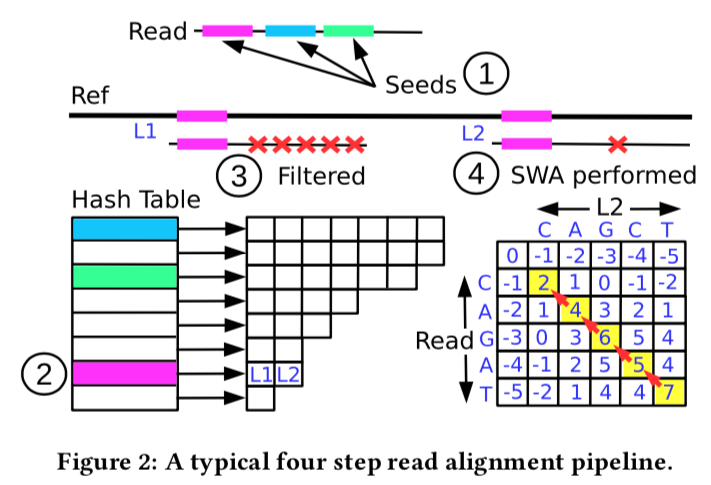
\includegraphics[scale=0.32]{fig/demo-steps.png}
\caption{A typical four step variant calling pipeline}
\label{fig:arch_design}
\end{figure}

\subsection{Variant calling algorithms}
Even though variant calling algorithms have been evolving and recently more and more algorithms have moved from position-based (\textit{e.g.} Mutect1~\cite{}) to graph-base (\textit{e.g.} HaplotypeCaller, Mutect2~\cite{}), and DNN-based algorithms (\textit{e.g.} applied somatic DeepVariant~\cite{}), most non-position-based algorithms are still being improved. 

%to write the distribution of three major pipelines
\subsection{Pair-HMM Algorithm}
this
\subsubsection{Algorithm description}
As a variant of Smith-Waterman algorithm, Pair-HMM is commonly used in variant-calling. The hidden Markov model is used in Pair-HMM to generate a probability score for the alignment between candidate haplotypes (H) and read sequences (R). Similar to Smith-Waterman algorithm, for a pair of nucleotides, there are three possibilities for one pair of sequences, i.e., match, insertion, and deletion. The The key difference is that Pair-HMM uses floating point operations.

The Pair-HMM algorithm takes a list of $N$ reads and a list of $M$ candidate haplotypes as input and returns the probability that the data would explain each one of the candidate haplotypes. To calculate the probability, the Pair-HMM performs assesses all possible alignments of each haplotype (the hypothesis) against all the reads (the data). The HMM has three main states: match, insertion and deletion. Here we introduce three concepts related to the base quality score ($Q_m$): The insertion gap open penalty (or base insertion quality $Q_i$), the deletion gap open penalty (or base deletion quality $Q_d$) and the gap continuation penalty ($Q_g$). The first two represent the probability that the base precedes an insertion or a deletion (respectively) and even when not reported by the instrument can be generated by the latest version of the Base Quality Score Recalibration tool (BaseRecalibrator) in the GATK [cite GATK]. The third represents the probability that an insertion or deletion are extended which in theory could be different for insertions and deletions, but in our model we use the same flat value $Q10$ for all gap continuation penalties.

\begin{figure}[htbp]
\centering
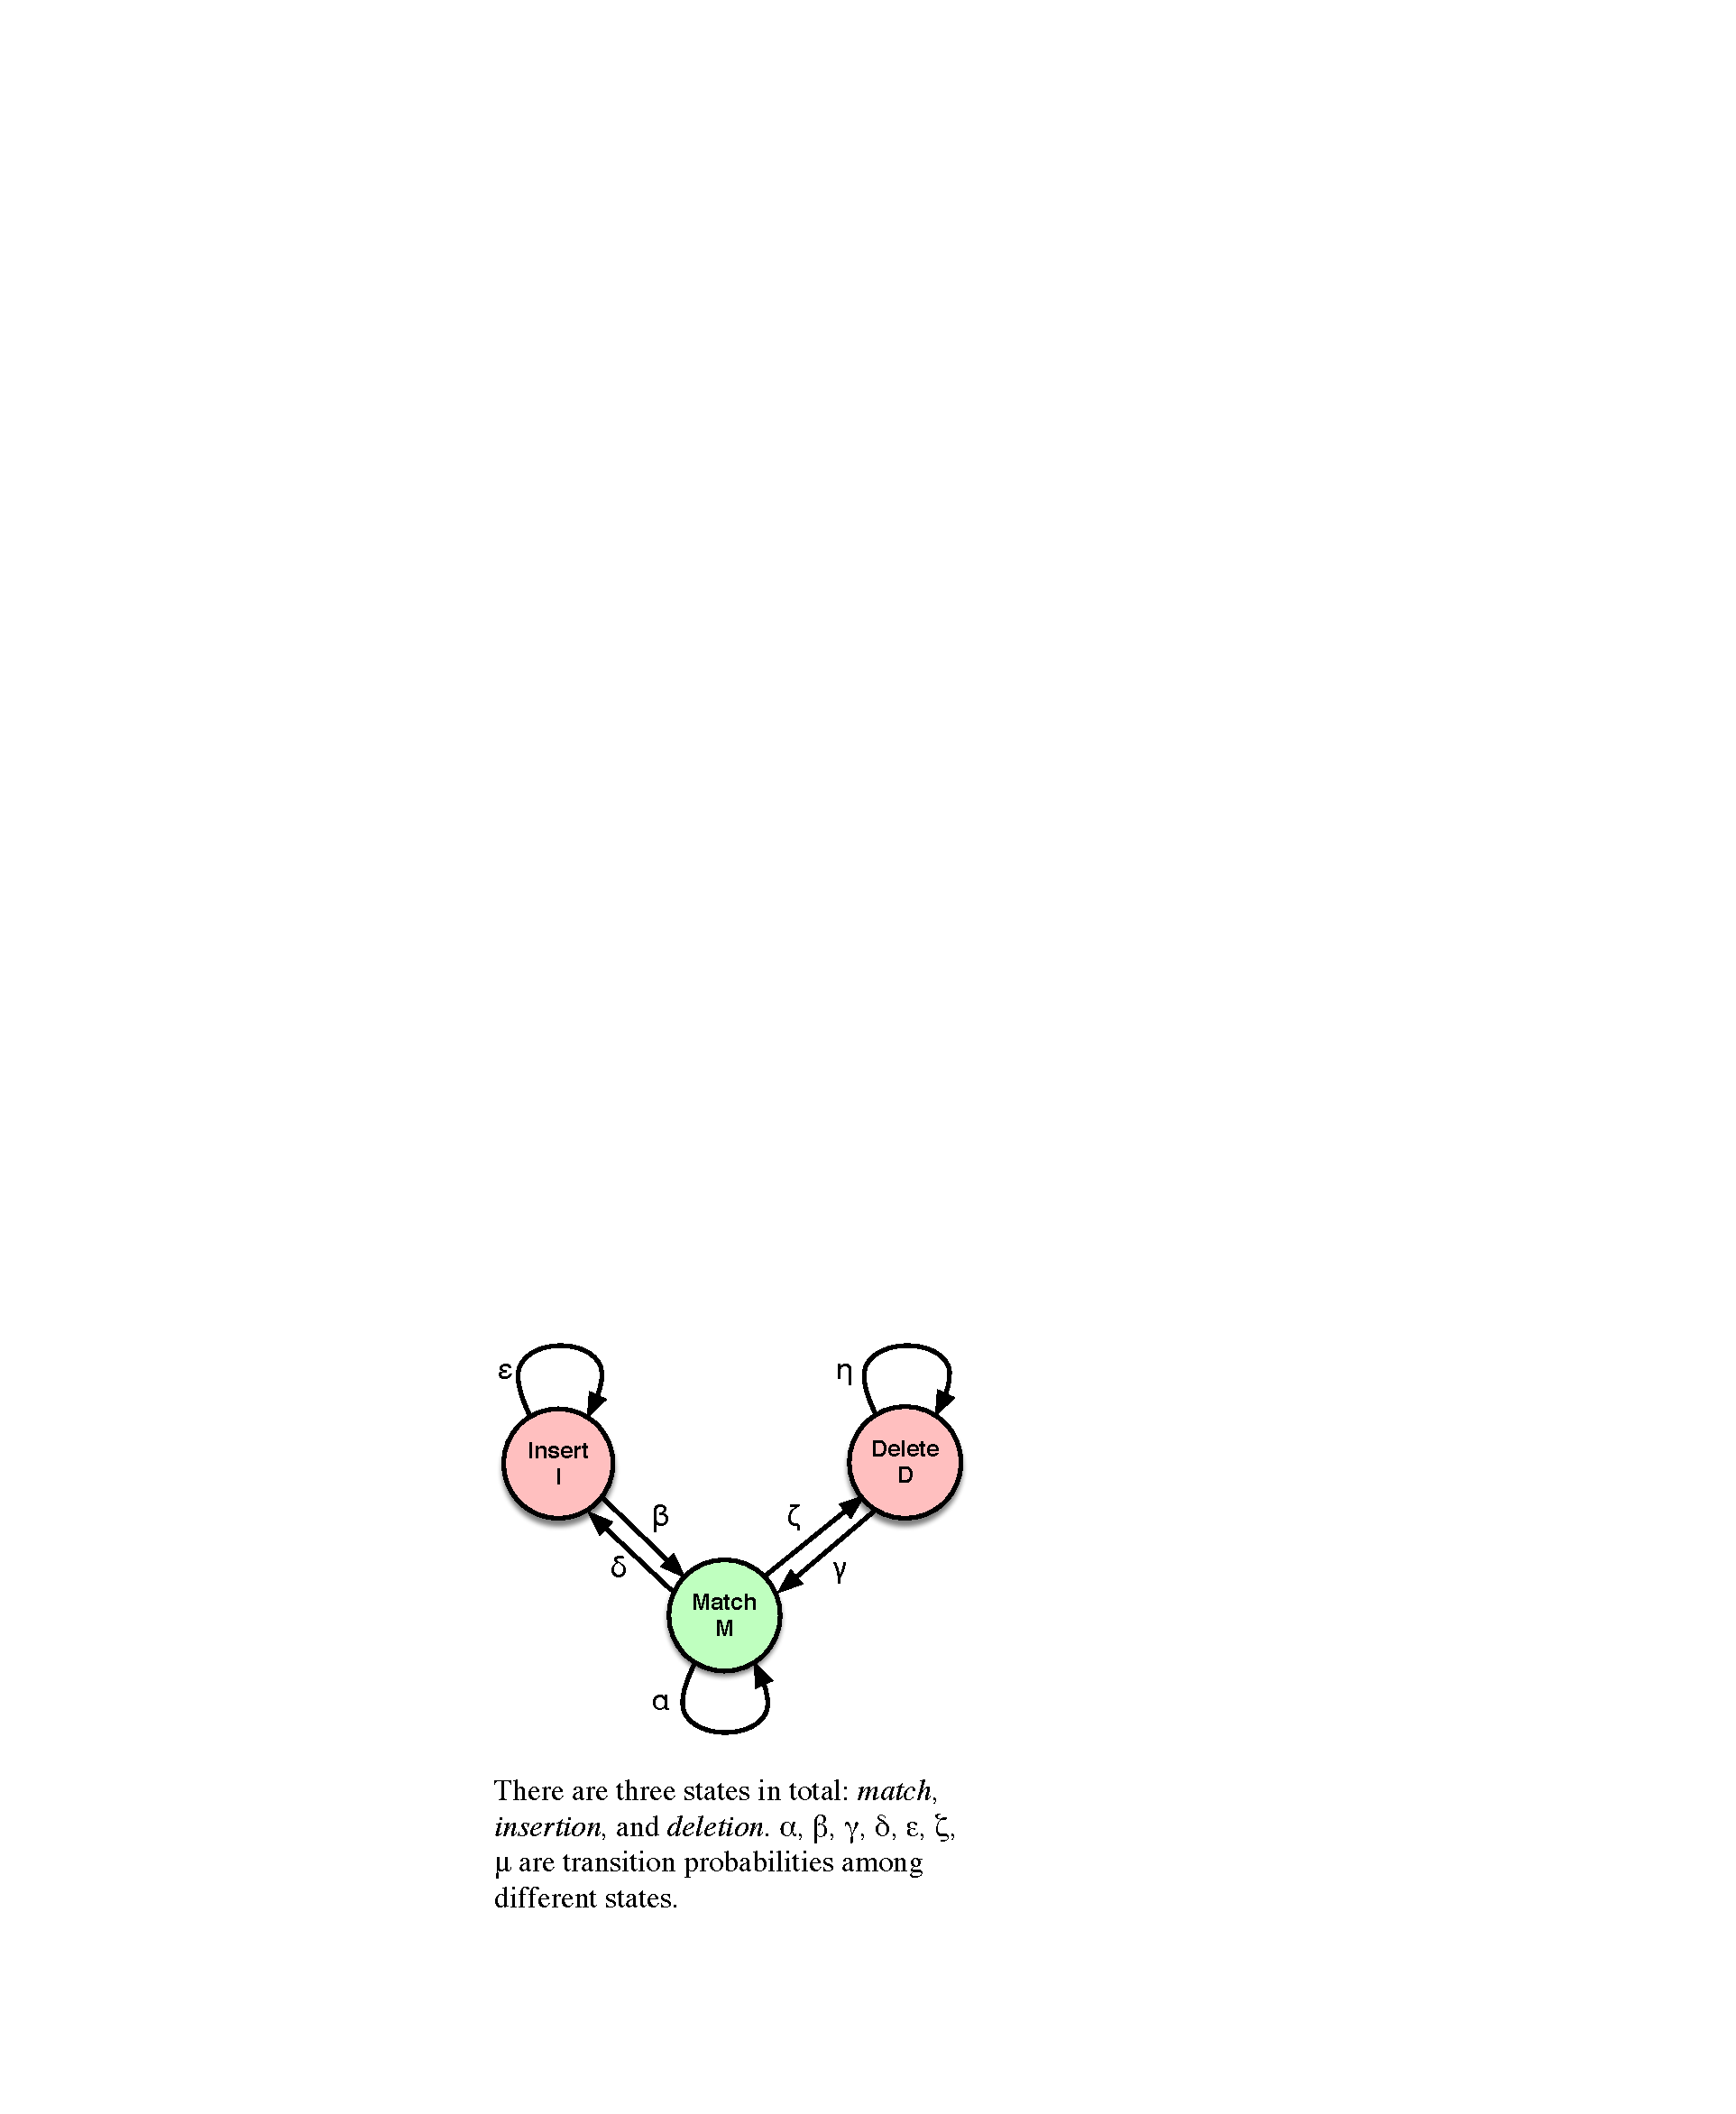
\includegraphics[scale=0.52]{fig/algo-pair-hmm.pdf}
\caption{Insert, delete, and match states of Pair-HMM.}
\label{fig:arch_design}
\end{figure}

The Pair-HMM accuracy relies on the accurate estimation of these four quality scores for every base. The Pair-HMM equations are described below:

\begin{align}
    M_{i,j} &= P_{i,j} (\alpha  M_{i-1,j-1} + \beta  I_{i-1,j-1} + \gamma D_{i-1,j-1} ) \\
    I_{i,j} &= \delta  M_{i-1,j} + \epsilon  I_{i-1,j} \\
    D_{i,j} &= \zeta   M_{i,j-1} + \eta  D_{i,j-1} 
\end{align}

Given that $Q_m$ is the base quality score of a base in the read converted from phred-scale to probability space using the formula $Q = -log_{10}P$. The prior $P_{i,j}$ is $1-Q_m$ of the $i^{th}$ base in the read if it matches the $j^{th}$ base in the haplotype, or $Q_m$ if it does not.  The transition probabilities are expressed by the roman letters in the equation and are described below: 

\begin{align*}
    \alpha   &= 1 - (Q_i + Q_d) \text{ | match continuation} \\
    \beta    &= 1 - Q_g \text{ | insertion to match} \\
    \gamma   &= 1 - Q_g \text{ | deletion to match} \\
    \delta   &= Q_i \text{ | match to insertion} \\
    \epsilon &= Q_g \text{ | insertion continuation} \\
    \zeta    &= Q_d \text{ | match to deletion} \\
    \eta     &= Q_g \text{ | deletion continuation}
\end{align*}

The resulting probability is theoretically the sum of $M_{N,M}$, $I_{N,M}$ and $D_{N,M}$, however there are a two special conditions in this HMM that change:

\begin{enumerate}

\item To allow the alignment of the haplotype to start anywhere on the read without penalty, we need to initialize the entire first row of the deletion matrix with the normalized factor $\frac{1}{\text{len(}R_i\text{)}}$.

\item To allow the alignment to end anywhere in the read without penalty, we need to ignore the last row of the deletion matrix ($D$) in the final calculation of the Pair-HMM probability.

\end{enumerate}

The key difference is that Pair-HMM uses floating point operations. For this study, we used our optimized implementation that is also a part of the Genomics Kernel Library (GKL) by Intel.

\subsubsection{Inter- and Intra-parallelism}

\begin{figure}[htbp]
\centering
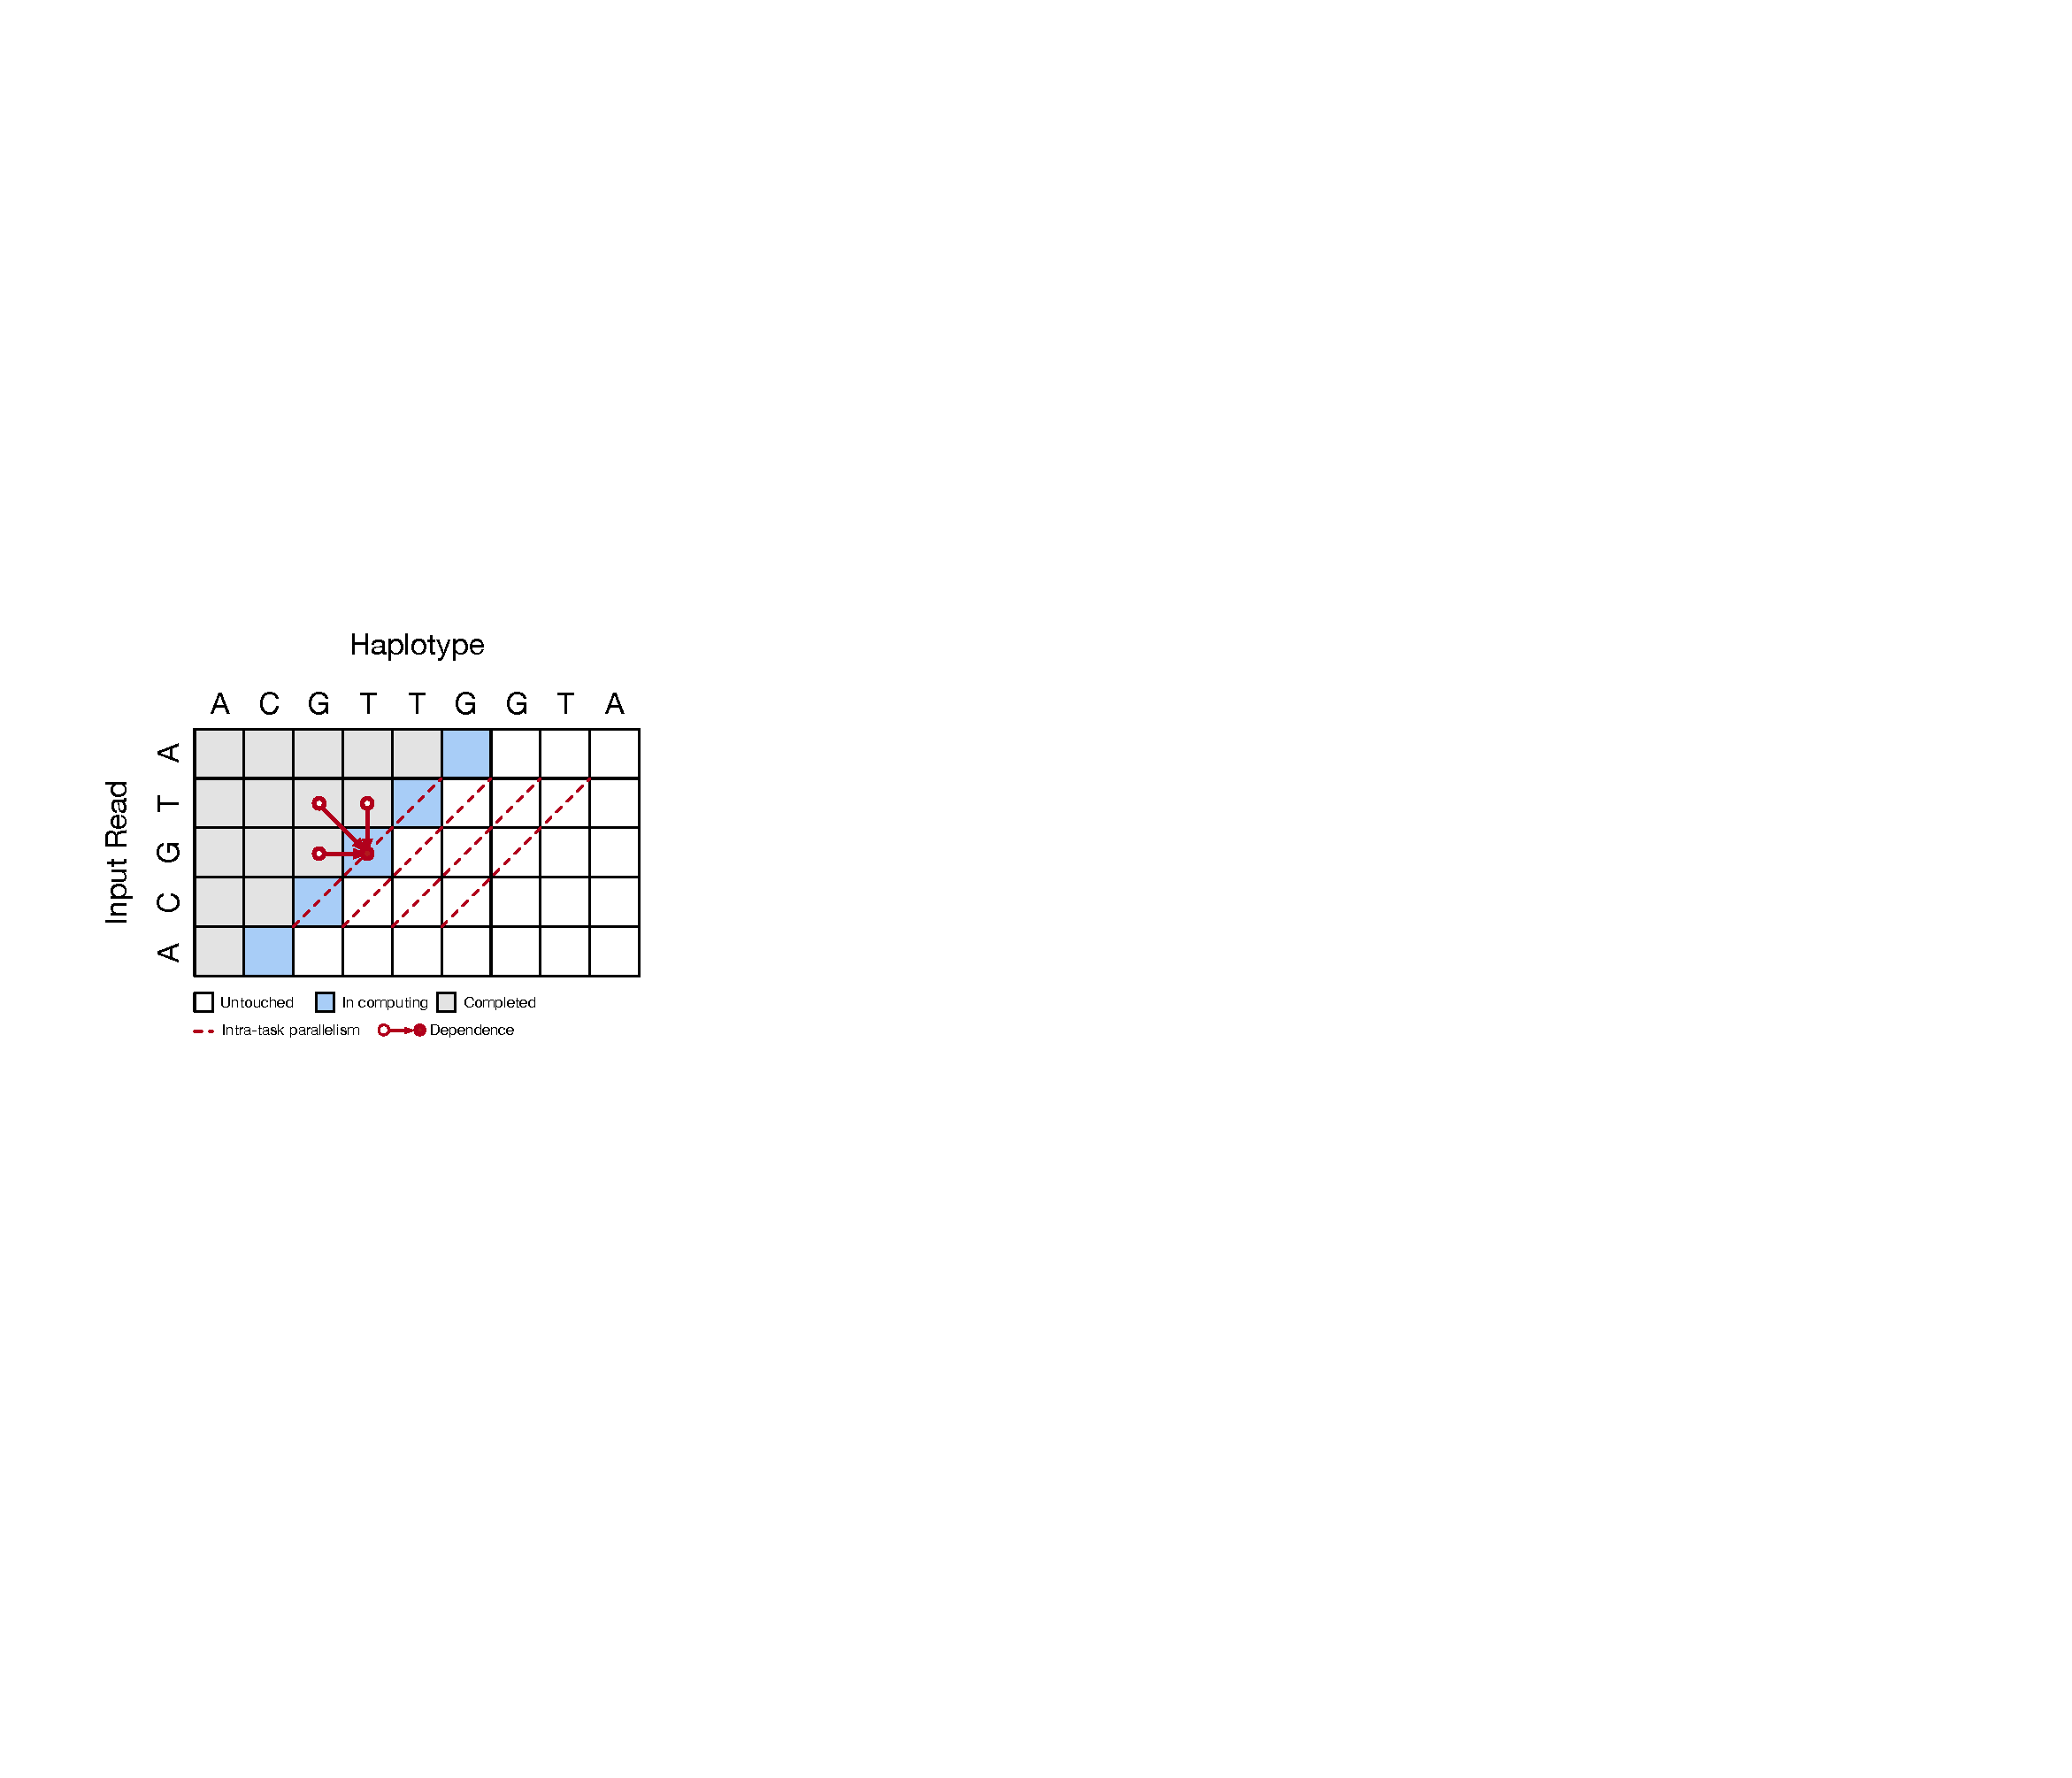
\includegraphics[width=\linewidth]{fig/algo-intra-parallelism.pdf}
\caption{}
\label{fig:para-pair-hmm}
\end{figure}


\subsection{Smith-Waterman}

%\section{INTRODUCTION}

%\newpage
\clearpage

%%%%%%% -- PAPER CONTENT ENDS -- %%%%%%%%

%%%%%%%%% -- BIB STYLE AND FILE -- %%%%%%%%
\bibliographystyle{ieeetr}
\bibliography{ref}
%%%%%%%%%%%%%%%%%%%%%%%%%%%%%%%%%%%%

\end{document}
